\documentclass[conference]{IEEEtran}
\usepackage{cite}
\usepackage{amsmath}
\usepackage{booktabs}
\usepackage{graphicx}
\usepackage{url}
\usepackage{array}
\begin{document}

\title{AXIVEX: A Modular 4$\times$4 Systolic-Array Accelerator for Matrix Multiplication}

\author{}

\maketitle

\begin{abstract}
AXIVEX is a synthesizable Verilog implementation of a 4$\times$4 output-stationary systolic array that computes
$C=AB$ for signed INT8 matrices with INT32 accumulation. This paper describes the array architecture, transaction
interface, verification methodology, browser Digital Twin, and open-source synthesis results. The RTL passes exhaustive
MAC-unit checks, directed unit and system tests, and a 128-transaction seeded random regression against an independent
Python model. Mutation testing detects all 18 non-equivalent injected faults. RTL simulation measures 13 cycles from
accepted start to completion, including a 10-cycle compute window in which the 16 processing elements perform 64
multiply-accumulate operations. Yosys mapping to Xilinx 7-series primitives reports 16 DSP48E1 blocks, 1,399 FDRE
registers, and 202 LUTs. These are resource-mapping results; no Vivado timing, maximum-frequency, power, or board
measurement is claimed. The Digital Twin visualizes cycle-level operation and is cross-validated against RTL traces.
\end{abstract}

\begin{IEEEkeywords}
systolic array, matrix multiplication, FPGA, Verilog, output-stationary dataflow, INT8
\end{IEEEkeywords}

\section{Introduction and Motivation}
Matrix multiplication dominates neural-network inference. A sequential engine with one multiply-accumulate (MAC) unit
needs $MNK$ cycles for an $M\times K$ by $K\times N$ product; a spatial array performs many MACs per cycle and reuses each
operand as it moves between neighbouring processing elements (PEs). AXIVEX is a small, fully verified instance of this idea,
built to be inspected, simulated and synthesized with free tools only.

\section{Literature Review}
Kung argued that systolic architectures, regular arrays in which data flows rhythmically through many PEs, allow multiple
computations per memory access and so suit compute-bound problems without raising I/O requirements \cite{kung1982}.
The Google TPU is a prominent production example: its core is a 65,536-MAC 8-bit matrix unit \cite{jouppi2017}.
Gemmini is an open-source generator of systolic accelerators with selectable dataflows and a full software stack \cite{genc2021}.
Eyeriss analyses dataflows for convolutional networks and proposes the row-stationary dataflow \cite{chen2016}.

\section{Existing Approaches and Limitations}
General-purpose cores execute matrix products with few MACs per cycle and repeated operand movement. Large accelerators
\cite{jouppi2017,genc2021} are valuable in production but can be difficult to inspect at the level of individual operand
transfers and accumulator updates. AXIVEX provides a smaller cycle-accurate implementation whose RTL, independent
reference model, test traces, and visualization describe the same fixed-size computation. Its deliberately narrow scope
also leaves important system-level challenges visible: the array is not parameterized, its packed interface is wide, and
its timing has not been characterized with a vendor implementation flow.

\section{Problem Statement}
Design, implement and verify in synthesizable Verilog a 4$\times$4 array computing $C_{4\times4}=A_{4\times4}B_{4\times4}$
with signed INT8 inputs and signed INT32 accumulation using 16 PEs, output-stationary dataflow, east-moving A and south-moving B.

\section{Proposed Solution}
\subsection{High-level architecture}
Fig.~\ref{fig:hld} shows the blocks: host interface, input buffers, skew scheduler, controller, 16-PE mesh and output buffer
(\texttt{rtl/}: nine modules). Data flows Host $\rightarrow$ input buffers $\rightarrow$ scheduler $\rightarrow$ PE mesh $\rightarrow$ output buffer $\rightarrow$ Host.
\begin{figure}[t]\centering
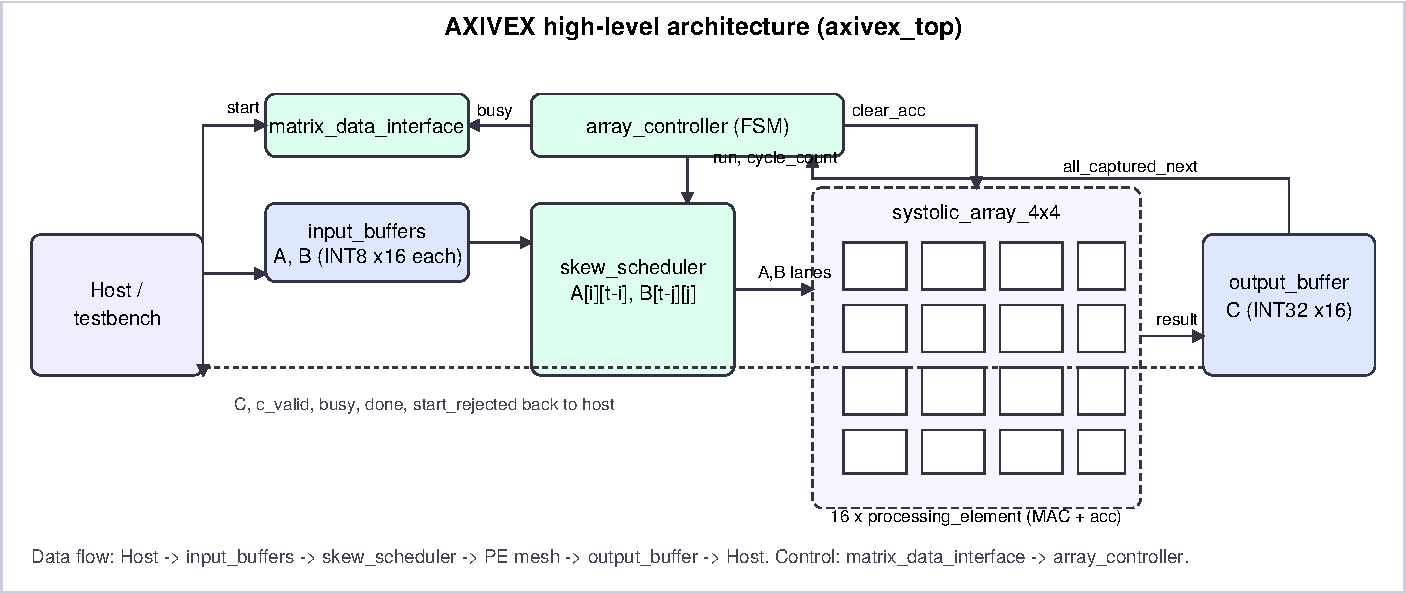
\includegraphics[width=\columnwidth]{../architecture/hld.pdf}
\caption{High-level architecture of \texttt{axivex\_top}.}\label{fig:hld}
\end{figure}

\subsection{PE microarchitecture}
Each PE holds registered copies of the A and B operands and their valid/last flags (one hop per clock), a 32-bit accumulator,
a result register and \texttt{result\_valid}. A MAC fires only when both operands are valid:
$acc\leftarrow acc+a\cdot b$, with the product sign-extended from 16 to 32 bits. When both last flags coincide the same sum is written to
the result register and \texttt{result\_valid} pulses once.

\subsection{Dataflow and schedule}
Row $i$ injects $A[i][k]$ at cycle $t=i+k$ and column $j$ injects $B[k][j]$ at $t=j+k$; both reach PE$(i,j)$ at
$t=i+j+k$. The final MAC of PE$(i,j)$ is at $t=K-1+i+j$, so the compute window is $K+M+N-2=10$ cycles and the last PE finishes at
$t=9$. Last markers travel with the operands instead of a global pulse, because the skew gives every PE a different final cycle.

\subsection{Controller}
IDLE $\rightarrow$ CLEAR (1 cycle) $\rightarrow$ RUN (10) $\rightarrow$ RETIRE (1) $\rightarrow$ DONE (1-cycle pulse). RETIRE ends when all 16
results are captured or arriving in that cycle, which counts simultaneous result pulses correctly.

\subsection{Arithmetic and numeric range}
Inputs use signed two's-complement INT8 representation. Multiplying two such operands produces an exact signed 16-bit
product, which is sign-extended before accumulation in a signed 32-bit register. For $K=4$, the largest positive output
is $4(-128)(-128)=65{,}536$; the most negative output is $4(-128)(127)=-65{,}024$. Both bounds fit comfortably in the
accumulator, so the supported operation needs no saturation or intermediate truncation. The PE forms the next sum from
the current accumulator and current product, then uses that same next sum for the final result. This detail preserves
the final product term when the last markers arrive.

\subsection{Top-level transaction interface}
The interface accepts two row-major packed 128-bit matrices and returns a row-major packed 512-bit result. Element
$A[i][k]$ occupies bits $8(4i+k)+:8$; $B[k][j]$ occupies bits $8(4k+j)+:8$; and $C[i][j]$ occupies bits
$32(4i+j)+:32$. A start rising edge is accepted only while the accelerator is idle. The input matrices are captured
on the accepting edge, so the source may change them during computation. The \texttt{busy} signal marks active
processing, \texttt{done} pulses for one cycle, and \texttt{c\_valid} indicates that all sixteen results are available.
An attempted start while busy is rejected and reported without disturbing the current transaction.

Reset is synchronous and active-low. It clears the controller, forwarding registers, accumulators, output buffer, and
valid state. The output buffer detects duplicate PE result pulses and raises a sticky error indication; the verification
environment checks that this signal remains deasserted during valid operation. The fixed-latency protocol has no
backpressure or mid-computation stall mechanism.

\section{Verilog Implementation}
The RTL is Verilog-2001 with explicit signed arithmetic, nonblocking assignments, synchronous active-low reset and flat packed ports
(row-major index $4i+j$). The design is divided into nine modules so that arithmetic, operand storage, schedule generation,
control, the PE mesh, and output capture can be simulated independently. Registered forwarding gives each PE one
registered hop per clock and keeps partial sums local. The skew scheduler derives the boundary inputs from the RUN
counter and matrix coordinates. This compact implementation is easy to inspect, but the counter-to-selection logic is
combinational and its impact on a realizable clock period has not been measured. Verilator \texttt{-Wall} lint is clean.
The interface and protocol contract are documented alongside the RTL.

\section{Dataflow and Cycle Accounting}
For a PE at row $i$, column $j$, the operands for reduction index $k$ meet at cycle $t=i+j+k$. The first product
therefore arrives at different cycles across the mesh, creating a diagonal wavefront. The last product for PE$(i,j)$
occurs at $t=K-1+i+j$; for a 4$\times$4 array, the final PE completes at cycle 9 of RUN. The RUN interval consequently
contains $K+M+N-2=10$ cycles: four cycles of useful reduction for each PE plus six cycles of wavefront fill and drain.

The array performs 64 MACs per matrix product. Counting active PEs by RUN cycle gives
1, 3, 6, 10, 12, 12, 10, 6, 3, and 1. The sum is 64, or an average of 6.4 active PEs during the ten-cycle compute
window. Relative to all 16 PEs, this is 40\% utilization in RUN. Including the load, clear, and retirement cycles
reduces utilization to 30.8\% over the measured start-to-completion interval. These measures describe array activity,
not an observed frequency or throughput in operations per second.

The cycle count is measured from the RTL testbench and reflects the controller protocol, not a theoretical lower bound.
A one-MAC baseline would require 64 sequential MAC operations for this same product. Dividing 64 by the ten-cycle
compute window yields a 6.4$\times$ compute-only ratio, but this baseline is analytical rather than an implemented
design and does not normalize for area, clock period, memory behavior, or interface overhead. It should not be
interpreted as an end-to-end speedup.

\section{Verification Methodology}
Testbenches written in SystemVerilog and run with Icarus Verilog cover the MAC, PE, output buffer, systolic array, and
top-level protocol. The MAC test enumerates all 65,536 pairs of signed INT8 operands over six accumulator seeds. PE
tests exercise valid and invalid input combinations, forwarding, accumulation, clear behavior, and the final result.
The array test drives a skewed operand wave and checks per-PE values and completion cycles; top-level tests check
transactions rather than only final arithmetic.

A cycle-by-cycle monitor checks valid and last-marker alignment, accumulation only when both operands are valid,
forwarding without data loss, one result per PE, and the absence of early completion. Directed vectors include identity,
zero, all-ones, signed values, diagonal and sparse matrices, INT8 extremes, and consecutive jobs. The top-level
scenarios also reset the design in IDLE, CLEAR, RUN, and RETIRE; attempt a start while busy; hold start high; and
launch back-to-back jobs. These cases exercise control behavior that a final-result comparison alone would not reveal.

An independent Python model computes $C[i][j]=\sum_k A[i][k]B[k][j]$ directly and produces deterministic reference
vectors. A seeded random regression runs 128 matrix pairs and compares the RTL outputs with this model. Keeping the
reference calculation structurally separate from the RTL reduces the risk of duplicating the same scheduling error in
both implementations. The simulator fixtures also provide recorded traces for the browser Digital Twin tests.

Mutation testing evaluates whether the test suite detects deliberately introduced RTL defects. The script injects
single-line changes such as altered arithmetic, control, forwarding, and validity behavior, then runs the relevant
regression. Eighteen non-equivalent mutants are detected; one additional mutant is documented as equivalent to the
reference behavior under the tested interface. This result is evidence about the test suite's sensitivity to those
mutations, not a proof of correctness for all possible inputs or implementations.

\section{Simulation Results}
\begin{table}[t]\centering\caption{Verification results (Icarus Verilog 12.0).}\label{tab:ver}
\begin{tabular}{@{}lr@{}}\toprule
Test & Result\\\midrule
MAC exhaustive & 393{,}218 checks, 0 errors\\
PE unit & 42 checks, 0 errors\\
Array & 77 jobs, 20{,}944 checks, 0 errors\\
Top, directed + scenarios & 35 jobs, 0 failures\\
Top, random & 128 jobs, 0 failures\\
Mutation check & 18/18 non-equiv. killed\\\bottomrule
\end{tabular}\end{table}
\begin{table}[t]\centering\caption{Cycle accounting (measured in RTL simulation).}\label{tab:cyc}
\begin{tabular}{@{}lr@{}}\toprule
Quantity & Value\\\midrule
Start-to-done latency & 13 cycles\\
\quad load/start, CLEAR, RUN, RETIRE & 1, 1, 10, 1\\
MACs per job & 64\\
Active PEs / RUN cycle & 1,3,6,10,12,12,10,6,3,1\\
PE utilization, RUN window & 40.0\%\\
PE utilization, start-to-done & 30.8\%\\
Single-MAC baseline & 64 cycles\\
Compute-only ratio & 6.4$\times$\\\bottomrule
\end{tabular}\end{table}
The single-MAC baseline is analytical, not implemented RTL, and the comparison is not area-normalised (16 MACs versus 1).
The recorded waveform shows operand wavefronts and anti-diagonal result pulses; multiple PEs may complete on the same
cycle, which is why the output buffer accepts multiple result events at once.

\section{Digital Twin}
The browser Digital Twin is a TypeScript model and visualization of the same fixed 4$\times$4 computation. Its engine
is separated from the React interface: the engine advances the design state cycle by cycle, while the pages and
components render inputs, processing elements, control state, registers, and outputs. This separation makes the model
usable in tests without a browser and keeps presentation logic from controlling the arithmetic schedule.

The simulator exposes example matrices and views for matrix input, mesh activity, clock progression, architecture,
registers, and results. Its tests check arithmetic and state transitions and compare simulated fields against committed
RTL traces. The Digital Twin suite contains 25 tests, and the engine reproduces every traced field of 21 RTL jobs; an
additional set of 149 Python vectors is used for cross-checking. These tests support consistency between the
model and recorded behavior, but they are not a formal equivalence proof between TypeScript and Verilog.

The Digital Twin is an educational and debugging aid, not a hardware executor. It does not communicate with an FPGA
or measure electrical timing. Its value is in making the schedule observable: a user can relate matrix coordinates to
the PE that owns each partial sum and follow the evolution of a transaction across cycles.

\section{Synthesis Results}
Yosys 0.33 with \texttt{synth\_xilinx -family xc7} maps the flattened design to Xilinx 7-series primitives. Table~\ref{tab:synth}
summarizes the principal counts in the committed utilization report. The LUT total is the sum of LUT2 through LUT6.
\begin{table}[t]\centering\caption{Flattened Yosys mapping to Xilinx 7-series primitives.}\label{tab:synth}
\begin{tabular}{@{}lr@{}}\toprule
Primitive & Count\\\midrule
DSP48E1 & 16\\
FDRE flip-flops & 1,399\\
LUT2--LUT6 & 202\\
CARRY4 & 6\\
BUFG & 1\\
Input buffers & 259\\
Output buffers & 517\\\bottomrule
\end{tabular}\end{table}

The packed interface itself has 259 input and 517 output signals including controls, clocks, and status. It exceeds the
user I/O capacity of the referenced Artix-7 device, so the current result is an out-of-context mapping, not a complete
pin-constrained board implementation. The Vivado Tcl flow is present but has not produced vendor utilization or timing
results. No maximum frequency, power, or measured board throughput is available.

\section{Evaluation Environment and Reproducibility}
The committed results were produced with Icarus Verilog 12.0 for simulation, Verilator 5.020 for lint, Yosys 0.33
for synthesis, and Node.js 22 for the browser simulator, on Ubuntu 24.04. The repository keeps the RTL, testbenches,
Python reference, input vectors, comparison traces, synthesis scripts, and reports together so that results can be
recreated from source rather than inferred from a presentation.

\begin{table}[t]\centering\small
\caption{Reproduction commands and principal outputs.}\label{tab:repro}
\resizebox{\columnwidth}{!}{%
\begin{tabular}{@{}p{.72in}p{.76in}p{1.72in}@{}}\toprule
Check & Command & Evidence\\\midrule
Regression & \texttt{make test} & RTL, Python, random tests, and lint\\
Synthesis & \texttt{make synth} & Generic and XC7 resource reports\\
Cycle report & \texttt{make bench} & Latency and utilization summary\\
Mutation & \texttt{make mutation} & Detection of injected faults\\
Twin tests & \texttt{npm test} & Engine and UI checks\\
Twin build & \texttt{npm run build} & Production bundle\\\bottomrule
\end{tabular}%
}
\end{table}

The vector generator uses a fixed seed (20261116) for the 128 random matrix pairs. Directed cases and generated
fixtures are stored in the repository, which makes the regression repeatable and allows changes to the model to be
compared against the same inputs. The RTL comparison script consumes recorded directed and random traces; the Digital
Twin tests use those fixtures to check simulation state as well as final matrix values. A developer can therefore
separate a numeric mismatch from a cycle-alignment mismatch.

The performance report derives cycle counts from RTL simulation state and observed MAC events. The 13-cycle latency
and ten-cycle RUN window are architectural measurements in simulation; they do not include a physical clock period.
The analytical single-MAC comparison is explicitly labeled as modeled and is not synthesized alongside AXIVEX. In
contrast, the Yosys primitive counts are outputs of a synthesis flow and describe mapped resources only. Keeping
these evidence types separate prevents simulation cycles, synthesis cell counts, and a modeled baseline from being
presented as if they were a single hardware benchmark.

The listed commands reproduce the project checks, but their scope has limits. Simulation does not model routed delay,
board I/O timing, or power. The mutation suite samples selected fault classes rather than all possible defects. The
Digital Twin trace comparison is finite, and the Python model is an independent implementation but not a formal
specification. Reproducibility supports review of the reported results; it does not remove the need for timing
constraints, formal properties, or board-level measurement in a larger implementation.

\section{Design Tradeoffs and Coverage}
Output-stationary operation was selected because it gives every matrix result a fixed location: PE$(i,j)$ owns
$C[i][j]$ for the duration of the transaction. This avoids moving partial sums between cells and makes the output
mapping direct. The operands, rather than the sums, move through registered links. Each input value can participate
in multiple products as it passes neighboring PEs, while each PE needs only its local accumulator and forwarding
registers.

The regular mesh also exposes the cost of a small array. For $M=N=K=4$, the 16 PEs perform 64 MACs, but the skewed
wavefront leaves some cells idle at the beginning and end of RUN. Adding more PEs without increasing the matrix size
would not improve this utilization automatically. Larger workloads would need a parameterized array, a tiling scheme,
or a different mapping to amortize the fill and drain cycles. Those choices would also increase the verification state
space and could require buffering and control not present in the current design.

The top-level interface favors simple, simultaneous matrix loading over pin efficiency. Two 128-bit operands and a
512-bit result make the simulator and testbench interface straightforward, but they exceed the user I/O of the
referenced FPGA package. A practical board interface would serialize or stream data, likely with a ready/valid
handshake. That change would affect latency and controller behavior, so it cannot be evaluated by treating the
existing 13-cycle result as an end-to-end system measurement.

The verification strategy combines local block tests with whole-transaction checks. Local tests isolate arithmetic
and storage behavior; array checks focus on spatial timing; top-level tests cover reset and start semantics; seeded
random cases broaden numeric coverage; and mutations test whether selected faults are observable. Table~\ref{tab:coverage}
summarizes how these evidence sources relate to the principal claims.

\begin{table}[t]\centering\small
\caption{Coverage evidence by design layer.}\label{tab:coverage}
\begin{tabular}{@{}p{.84in}p{1.14in}p{1.18in}@{}}\toprule
Layer & Main check & Reported result\\\midrule
MAC & Signed operand and accumulator combinations & 393,218 checks; 0 errors\\
PE / storage & Validity, accumulation, clear, and result handling & Directed unit checks pass\\
Array & Skew, forwarding, and per-PE completion & 77 jobs; 20,944 checks pass\\
Top level & Reset, busy start, held start, consecutive jobs & 35 directed jobs pass\\
Random & RTL output versus Python reference & 128 seeded jobs match\\
Digital Twin & UI/engine tests and RTL traces & 25 tests; 21 jobs cross-checked\\
Mutation & Deliberate non-equivalent RTL faults & 18 of 18 detected\\\bottomrule
\end{tabular}\end{table}

No single row establishes correctness by itself. Exhaustive MAC testing checks a bounded arithmetic block, while the
array and top-level checks exercise timing and protocol interactions. Random testing can expose combinations missing
from hand-written vectors but does not prove completeness. Mutation results depend on the selected faults. Together,
the checks provide complementary evidence for the stated fixed-size behavior and make it easier to localize a failure
to arithmetic, data movement, control, or visualization.

\section{Discussion and Limitations}
AXIVEX demonstrates an end-to-end design path from a specified dataflow to RTL, simulation, a reference model, synthesis
reports, and an interactive model. Its fixed dimensions make cycle accounting and verification manageable, and the
output-stationary organization gives each result a direct owner in the PE mesh. The same fixed scope limits reuse: the
matrix dimensions and reduction length are hard-coded, and the packed interface is suitable for simulation and
out-of-context synthesis rather than direct connection to a small FPGA package.

Several important measurements remain open. Yosys resource counts do not predict a validated clock frequency.
The combinational path from the scheduler counter through input selection and multiplication needs timing analysis.
The design has no stalls or backpressure, no gate-level simulation, and no power measurement. The 6.4$\times$ ratio
compares only compute-window cycles against a modeled one-MAC engine and is neither area-normalized nor a measured
system-level speedup. The Digital Twin is regression-tested against traces but has not been formally proven equivalent
to the RTL. These limitations define the boundary of the results presented here.

Useful extensions include parameterizing array dimensions and reduction length, narrowing the external interface,
adding a handshake or streaming protocol, and evaluating tiling or double buffering. A vendor timing run and a
measured baseline would enable a more complete performance comparison. Such extensions require new verification and
should be reported with measured results rather than inferred from the existing resource mapping.

\section{Conclusion}
A 4$\times$4 output-stationary systolic multiplier was implemented and verified in simulation against an independent
reference model. Its measured transaction latency is 13 cycles, with a ten-cycle compute window for 64 MACs. Yosys
produces a reproducible mapping to 16 DSP48E1 blocks, 1,399 FDRE registers, and 202 LUTs. The Digital Twin provides a
cycle-level view of the same computation, while the test suite covers arithmetic, data movement, control, and randomized
transactions. Timing, frequency, power, and board-level performance remain unmeasured; the report therefore presents
resource counts and cycle counts without claiming a clock-rate or end-to-end speedup.

\begin{thebibliography}{1}
\bibitem{kung1982} H. T. Kung, ``Why systolic architectures?,'' \emph{Computer}, vol. 15, no. 1, pp. 37--46, Jan. 1982, doi: 10.1109/MC.1982.1653825.
\bibitem{jouppi2017} N. P. Jouppi \emph{et al.}, ``In-datacenter performance analysis of a tensor processing unit,'' in \emph{Proc. 44th Annu. Int. Symp. Comput. Archit. (ISCA)}, Toronto, ON, Canada, 2017, pp. 1--12, doi: 10.1145/3079856.3080246.
\bibitem{genc2021} H. Genc \emph{et al.}, ``Gemmini: Enabling systematic deep-learning architecture evaluation via full-stack integration,'' in \emph{Proc. 58th ACM/IEEE Design Autom. Conf. (DAC)}, 2021, pp. 769--774, doi: 10.1109/DAC18074.2021.9586216; arXiv:1911.09925.
\bibitem{chen2016} Y.-H. Chen, J. Emer, and V. Sze, ``Eyeriss: A spatial architecture for energy-efficient dataflow for convolutional neural networks,'' in \emph{Proc. 43rd Int. Symp. Comput. Archit. (ISCA)}, 2016, pp. 367--379, doi: 10.1109/ISCA.2016.40.
\bibitem{iverilog} S. Williams, ``Icarus Verilog.'' [Online]. Available: https://steveicarus.github.io/iverilog/ (software documentation).
\bibitem{yosys} C. Wolf, ``Yosys open synthesis suite.'' [Online]. Available: https://yosyshq.net/yosys/ (software documentation).
\end{thebibliography}
\end{document}
